\documentclass[10 pt,usenames,dvipsnames, oneside]{article}
\usepackage{../../../modelo-ensino-medio}



\begin{document}

\begin{center}
  \begin{minipage}[l]{3cm}

\includegraphics[width=2cm]{logo}    
\end{minipage}\hfill
\begin{minipage}[r]{.8\textwidth}
 {\Large \scshape Atividade: Distributividade}  
\end{minipage}
\end{center}
\vspace{.2cm}

\ifdefined\prof
%Habilidades da BNCC
\begin{objetivos}
\item a
\end{objetivos}

%Caixa do Para o Professor
\begin{goals}
%Objetivos específicos
\begin{enumerate}
\item Verificar a propriedade distribuitiva da operação 
\end{enumerate}

\tcblower

%Orientações e sugestões
\begin{itemize}
\item Dois diagramas de venn são apresentados. A ideia é realizar a verificação pintando os diagramas conforme a operação à esquerda e à direita da igualdade, para concluir que se referem ao mesmo conjunto.
\end{itemize}
\end{goals}

\bigskip
\begin{center}
{\large \scshape Atividade}
\end{center}
\fi

Verifique, usando os diagramas de Venn na \hyperref[diagramavenn3]{figura \ref{diagramavenn3}}, a propriedade distributiva da operação de união com a interseção de dois conjuntos.
\begin{equation*}
\begin{split}(A\cap B)\cup C=(A\cup C)\cap (B\cup C)\end{split}
\end{equation*}

\begin{figure}[H]
\centering
\begin{minipage}{0.35\textwidth}
\centering
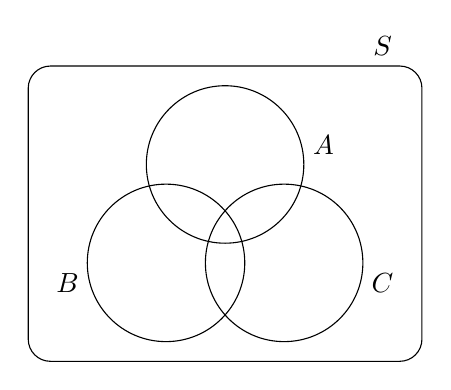
\begin{tikzpicture}[scale=0.5, every node/.style={scale=1}]
\draw [,rounded corners=8pt,] (0,0) -- (0,7.5) -- (10,7.5) -- (10,0) -- cycle;
\node  at (9,8) {$S$};
\draw (3.5,2.5) circle (2cm);
\node  at (1,2) {$B$};
\draw (6.5,2.5) circle (2cm);
\node  at (9,2) {$C$};
\draw (5,5) circle (2cm);
\node  at (7.5,5.5) {$A$};
\end{tikzpicture}

\end{minipage}
\begin{minipage}{0.35\textwidth}
\centering
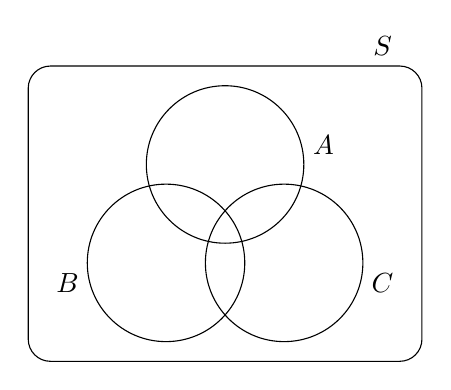
\begin{tikzpicture}[scale=0.5, every node/.style={scale=1}]

\draw [,rounded corners=8pt,] (0,0) -- (0,7.5) -- (10,7.5) -- (10,0) -- cycle;
\node at (9,8) {$S$};
\draw (3.5,2.5) circle (2cm);
\node at (1,2) {$B$};
\draw (6.5,2.5) circle (2cm);
\node at (9,2) {$C$};
\draw (5,5) circle (2cm);
\node at (7.5,5.5) {$A$};
\end{tikzpicture}

\end{minipage}
\caption{Diagramas de Venn com três conjuntos: \(A\), \(B\)  e \(C\)}
\label{diagramavenn3}
\end{figure}

\ifdefined\prof
\clearpage
\begin{solucao}
\begin{figure}[H]
\centering

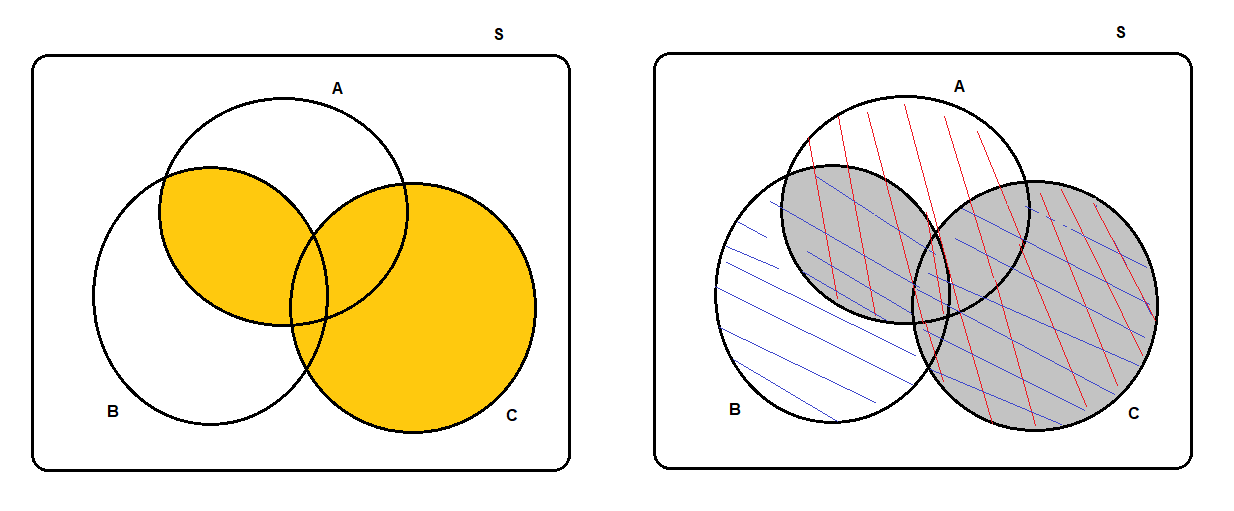
\includegraphics[width=\linewidth]{distributividade.png}
\caption{Diagramas de Venn: $(A\cap B)\cup C=(A\cup C)\cap(B\cup C)$}
\label{}
\end{figure}

No diagrama da esquerda tem-se em amarelo a região indicada pela expressão à esquerda na igualdade a ser verificada. No diagrama da direita tem-se $A\cup C$ em listras vermelhas, $B\cup C$ em listras azuis. A região da interseção dos dois é a que contêm listras azuis e vermelhas e está destacada na cor cinza. Observe que é a mesma região em amarelo do diagrama da esquerda.

\end{solucao}
\fi

\end{document}